% This work is licensed under the Creative Commons
% Attribution-NonCommercial 3.0 Unported License. To view a copy of this
% license, visit http://creativecommons.org/licenses/by-nc/3.0/.

% This work is licensed under the Creative Commons
% Attribution-NonCommercial 3.0 Unported License. To view a copy of this
% license, visit http://creativecommons.org/licenses/by-nc/3.0/.

% ==========================================================================
%                     Festlegung der Dokumentenklasse
% ==========================================================================

% Dokumentklasse für Aufsätze, Berichte, etc.
\documentclass[paper=a4, german, titlepage]{scrartcl}

% Behebt ein paar Fehler in Latex
\usepackage{fixltx2e}

% ==========================================================================
%                            Detailtypographie
% ==========================================================================

\usepackage{microtype}

% ==========================================================================
%                             Zeichenkodierung
% ==========================================================================

% UTF-8 als Eingabe-Kodierung und T1 als Fontkodierung
\usepackage[utf8]{inputenc}
\usepackage[T1]{fontenc}

% ==========================================================================
%                               Schriftarten
% ==========================================================================

\usepackage{lmodern}

\setkomafont{disposition}{\normalfont\bfseries}

% ==========================================================================
%                           Spracheinstellungen
% ==========================================================================

% Deutsche Zeichenketten
\usepackage[german]{babel}


% ==========================================================================
%                        Bibliograhphie und Anhang
% ==========================================================================

\newcommand{\theappendix}{
  \clearpage
  \appendix
}

% Deutsche Guillemets mit \enquote{}
\usepackage[german=guillemets]{csquotes}

\usepackage[style=numeric-comp, backend=biber]{biblatex}
\bibliography{../literatur.bib}

% Nachnamen in Kapitälchen
\renewcommand*{\mkbibnamelast}[1]{\textsc{#1}}

% ==========================================================================
%                    Grafiken, Abbildungen und Tabellen
% ==========================================================================

% Verwenden von Farben und Grafiken
\usepackage{graphicx}
\usepackage{xcolor}

% Einbinden von ganzen PDF-Seiten
\usepackage{pdfpages}

% kleine Schrift für Bildunterschriften, Fettgedruckte Bildunterschriften
\usepackage[font=small,	labelfont=bf, format=plain]{caption}

% Für mehrere Objekte nebeneinander mit eigenen Bildunterschriften
\usepackage{subcaption}

% Beinhaltet \FloatBarrier , sodass nach diesem Befehl keine Floats mehr erscheinen
\usepackage[section]{placeins}

% Text umläuft Fließobjekte
%\usepackage{wrapfig}

% Tabellensatz
% \usepackage{tabularx}
\usepackage{booktabs}
\usepackage{longtable}

% Zum Verdrehen von Objekten. Nur mäßig verwenden.
% \usepackage{rotating}

% Setzen des Pfades für eingebundene Bilder
% \graphicspath{{figs/}{bilder/}}

% ==========================================================================
%                    Mathematikumgebungen und Einheiten
% ==========================================================================

% Paket für mathematische Umgebungen und Funktionen
\usepackage[intlimits]{amsmath}

% Zusätzliche Mathematische Schriftarten
\usepackage{amsfonts}

% Zusätzliche Mathematische Symbole
\usepackage{amssymb}

% Zum Setzen Kommutativer Diagramme
% \usepackage{amscd}

% Textsatz in der Matheumgebung
\usepackage{amstext}

% Aufrechte griechische Buchstaben
%\usepackage{upgreek}


% Diagramme mit tikz und Gnuplot zeichnen
% \usepackage{tikz}
% \usepackage{tikz-qtree}
% \usepackage{gnuplot-lua-tikz}

% ==========================================================================
%               automatischer Satz von Einheiten mit SIUnitX
% ==========================================================================

\usepackage[
% Stellt den Fehler separat dar: Siehe SIUnitX-Manual
  separate-uncertainty = true,
]{siunitx}

% Babel stellt SIUnitX auf deutsch ein, wenn german gewählt wird
\addto\extrasgerman{\sisetup{locale = DE}}

% Kürzen von Einheiten in SIUnitX ermöglichen
% \usepackage{cancel}

% ==========================================================================
%                  Aufzählungen, Referenzen und Links
% ==========================================================================

\usepackage{enumitem}

% Formattiert URLs, so dass sie sich z.B. besser vom Text abheben
\usepackage{url}

% TrueType-Schrift für URLs
% \urlstyle{tt}


% Verlinkungen innerhalb und außerhalb des PDF-Dokuments
\usepackage[colorlinks=false]{hyperref}

% intelligente Verlinkungen
\usepackage{cleveref}

% ==========================================================================
%                            Textsatzparameter
% ==========================================================================

% Vermeidung von "Schusterjungen" Höchstwert 10000, dann dürfen
% theoretisch keine Schusterjungen mehr auftreten.
\clubpenalty = 3000
% Vermeidkung von "Hurenkindern" Höchstwert 10000, dann dürfen
% theoretisch keine Hurenkinder mehr auftreten.  Es werden beide
% Einstellungen benötigt.
\widowpenalty = 3000
\displaywidowpenalty = 3000

% This work is licensed under the Creative Commons
% Attribution-NonCommercial 3.0 Unported License. To view a copy of this
% license, visit http://creativecommons.org/licenses/by-nc/3.0/.

% Differentialrechnung
\renewcommand{\d}{\ensuremath{\mathrm{d}}}

% Totale Ableitungen
\newcommand{\td}[2]{\ensuremath{\frac{\d{#1}}{\d{#2}}}}
\newcommand{\tdd}[2]{\ensuremath{\frac{\d^2{#1}}{\d{#2}^2}}}

% Partielle Ableitungen
\newcommand{\pd}[2]{\ensuremath{\frac{\partial{#1}}{\partial{#2}}}}
\newcommand{\pdd}[2]{\ensuremath{\frac{\partial^2{#1}}{\partial{#2}^2}}}

% Der Körper der reellen Zahlen
\newcommand{\R}{\ensuremath{\mathbb{R}}}

% Der Körper der komplexen Zahlen
\newcommand{\C}{\ensuremath{\mathbb{C}}}

% Imaginäre Einheit
\newcommand{\iu}{{\mathrm{i}\mkern1mu}}

\newcommand{\name}[1]{\textsc{#1}}

\titlehead{{TU Dortmund \hfill SS~13\\}
Fakultät Physik\\
Experimentelle Übungen II}

\subject{Versuchsprotokoll}
\title{Messung der Suszeptibilität paramagnetischer Substanzen}
\subtitle{Versuch 606}

\author{Daniel Meißner\\
{\normalsize\url{daniel.meissner@udo.edu}}
\and
Kevin Moch\\
{\normalsize\url{kevin.moch@udo.edu}}}

\date{06. Juni 2013}

\begin{document}
\maketitle

\tableofcontents
\clearpage

% This work is licensed under the Creative Commons
% Attribution-NonCommercial 3.0 Unported License. To view a copy of this
% license, visit http://creativecommons.org/licenses/by-nc/3.0/.

\section{Einleitung}
In diesem Versuch soll die Reichweite von $\alpha$-Strahlung in Luft
bestimmt werden. Dazu wird die mittlere Reichweite der
$\alpha$-Strahlung bei verschiedenen Drücken bestimmt. Anschließend wird
die Statistik des radioaktiven Zerfalls überprüft.

% This work is licensed under the Creative Commons
% Attribution-NonCommercial 3.0 Unported License. To view a copy of this
% license, visit http://creativecommons.org/licenses/by-nc/3.0/.

\section{Theorie}
%
\subsection{Leitungselektronen im Metall}
%
Metalle bestehen aus Atomen, von denen fast alle ionisert sind, und
welche ein Kristallgitter bilden. Die von den Atomen freigegebenen
Elektronen bewegen sich zwischen den Ionenrümpfen.  Das Gitterpotential,
welches durch diese Ionenrümpfe erzeugt wird, kann in einer schlichten
Näherung als konstant angesehen werden, sodass sich das Modell des
Potentialtopfes für das Atomgitter ergibt. Die Elektronen müssen in
diesem Modell eine Energie besitzen, die größer ist als die Tiefe des
Potentialtopfes multipliziert mit der Elementarladung.

Die Quantenmechanik liefert Aussagen über die Energie der
Leitungselektronen.  Elektronen sind Fermionen, besitzen also einen
halbzahligen Spin. Daher greift für Elektronen das \name{Pauli}-Prinzip,
welches besagt, dass es keine zwei Elektronen im Metallverband gibt, die
sich im selben Zustand befinden. Da es zwei mögliche Spins,
$\frac{1}{2}$ und $-\frac{1}{2}$, für Elektronen gibt bedeutet dies,
dass es pro Energie nur zwei Elektronen gibt, die diese Energie
besitzen.

Des weiteren folgt aus der Quantenmechanik bei der Betrachtung von
Elektronen im Potentialtopf, dass diese Elektronen nur diskrete Energien
besitzen können. Die größtmögliche Energie, die ein Elektron im Metall
am absoluten Nullpunkt haben kann, wird als \name{Fermi}sche
Grenzenergie $\zeta$ bezeichnet.

Die Wahrscheinlichkeit, ein Elektron mit der Energie $E$ im Metall mit
der Temperatur $T$ im thermischen GLeichgewicht zu finden, wird durch
die \name{Fermi}-\name{Dirac}-Verteilung beschrieben, welche in
Formel~\eqref{eq:fermi_dirac} wiedergegeben ist.
\begin{equation}
f(E) = \frac{1}{\exp{\left(\frac{E - \zeta}{kT}\right)}+1}
\label{eq:fermi_dirac}
\end{equation}
%
\subsection{Kennlinie einer Hochvakuum-Diode}
%
In diesem Versuch wird eine Hochvakuum-Diode verwendet, um die
Austrittsarbeit von Wolfram zu bestimmen. In Abb.~\ref{fig:diode} ist
ein Schaltbild zu sehen, in welcher der grundsätzliche Aufbau dieses
Versuchs skizziert ist.  Das zu untersuchende Metall dient als Kathode
und wird erhitzt. Die aus dem Metall gelösten Elektronen werden durch
eine Beschleunigungsspannung zur Anode hin beschleunigt. Der fließende
Strom wird gemessen. Die Beschleunigungsspannung aufgetragen gegen die
Stromsärke wird als Kennlinie der Hochvakuumdiode bezeichnet.  In
Abb.~\ref{fig:diode} ist eine solche Kennlinie zu sehen.  Das
Zustandekommen der verschiedenen Gebiete wird in den nachfolgenden
Sektionen erklärt.
%
\begin{figure}[]
\centering
\includegraphics[height = 3 cm]{diode}
\hspace{7 mm}
\includegraphics[height = 4 cm]{kennlinie}
\caption{Links zu sehen ist das Schaltbild einer Hochvakuumdiode. Rechts
  befindet sich der theoretische Verlauf der Kennlinie einer
  Hochvakuumdiode. Entnommen aus \textcite{v504}}
\label{fig:diode}
\end{figure}
%

\subsubsection{Das Anlaufstromgebiet}
%
Das Anlaufstromgebiet befindet sich bei der Kennlinie bei negativer
Beschleunigungsspannung. Dies bedeutet also, dass auch bei einer
angelegten Gegenspannung Elektronen bis zur Anode gelangen.

Dies ist damit zu erklären, dass es nach der
\name{Fermi}-\name{Dirac}-Verteilung in~\eqref{eq:fermi_dirac}
Elektronen im Metall gibt, die bei einer Temperatur $T > 0$ eine
Energiebesitzen, mit der sie das Metall verlassen können und noch eine
kinetische Energie außerhalb der Metalls besitzen, mit welcher die
Elektronen gegen die Gegenspannung anlaufen können. Daher rührt auch der
Name des Anlaufgebietes.

Außerdem besitzt das Anodenmaterial eine größere Austrittsarbeit, sodass
sich durch die elektrische Verbindung der Kathode mit der Anode
außerhalb der Diode bereits ein Gegenfeld bei nicht eingestellter
Spannung bildet. Für große Energien verhält sich die
Verteilung~\eqref{eq:fermi_dirac} exponentiel fallend, sodass sich die
Kennlinie im Bereich des Anlaufstromgebietes exponentiell steigend
verhalten muss.

Die Stromdichte im Anlaufstromgebiet ergibt sich zu dem in
Formel~\eqref{eq:anlaufstromdichte} wiedergegeben Ausdruck.
\begin{equation}
\text{const}\exp{\left(-\frac{e_0V}{kT}\right)}
\label{eq:anlaufstromdichte}
\end{equation}
%
\subsubsection{Das Raumladungsgebiet}
%
Da die Elektronen im elektrischen Feld der Diode gleichmäßig
beschleunigt werden und innerhalb der Diode nicht abgebremst werden,
gilt hierbei nicht das \name{Ohm}sche Gesetz, sodass sich auch kein
linearer Zusammenhang zwischen Spannung und Stromstärke einstellt.

Um den Verlauf der Kennlinie im Raumladungsgebiet, also für positive
Spannungen, welche noch nicht in den Sättigungsbereich gehen, zu
erhalten, werden die Kontinuitätsgleichung und die Poissongleichung
verwendet.

Das Ergebnis dieser Rechnung wird als
\name{Langmuir}-\name{Schottky}sche Raumladungsgleichung bezeichnet und
ist in Formel~\eqref{eq:raumladung} wiedergegeben. Dabei bezeichnet $j$
die Stromdichte, $V$ die angelegte Spannung und $a$ den Abstand zwischen
Kathode und Anode.
\begin{equation}
j = \frac{4}{9} \epsilon_0 \sqrt{2e_0/m_0} \frac{V^{\frac{3}{2}}}{a^2}
\label{eq:raumladung}
\end{equation}
%
\subsubsection{Das Sättigungsstromgebiet}
%
Das Sättigungsstromgebiet beginnt ab der Spannung, ab der ein Wendepunkt
in der Kennlinie auftritt. Dieses Gebiet kommt dadurch zustande, dass
bei einer festen Temperatur $T$ der Kathode pro Zeit und Fläche eine
endliche Menge an Elektronen aus der Metalloberfläche
austreten. Folglich kann also pro Zeit und Fläche nur maximal diese
Anzahl von Elektronen an der Anode ankommen.

Um eine Formel für die Anzahl der austretenden Elektronen pro Zeit und
Fläche aus der Kathode, also derSättigungsstromdichte $j_S$, zu
erhalten, wird die
\name{Fermi}-\name{Dirac}-Verteilung~\eqref{eq:fermi_dirac} für große
Energien der Elektronen betrachten.  Anschließend werden alle Elektronen
pro Zeit und Fläche gezählt, die eine eine Geschwindigkeitskomponente
senkrecht zur Metalloberfläche besitzen, welche ausreicht, um das Metall
zu verlassen. Multipliziert man die erhaltene Anzahl mit der
Elementarladung $e_0$, ergibt sich die gesuchte Formel, welche
\name{Richardson}-Gleichung genannt wird und in
Formel~\eqref{eq:richard} angegeben ist. $T$ ist die Temperatur, $k$ die
\name{Boltzmann}-Konstante und $\phi$ das Austrittspotential.
%
\begin{equation}
j_S(T) = 4\pi\frac{e_0m_0k^2}{h^3}T^3\exp{\left(\frac{-e_0\phi}{kT}\right)}
\label{eq:richard}
\end{equation}
%

\section{Durchführung}
\label{sec:Durchführung}
\begin{figure}[h]
	\centering
	\includegraphics[width=14cm,height=11cm]{fotos/Bilddurchfuhrung1.pdf}
	\caption{Schematischer Aufbau der Messapparatur}
	\label{durch:1}
\end{figure}
Zuerst soll eine Vorbereitungsaufgabe gelöst werden, um mit der Durchführung beginnen zu können.
Als erstes wird die Cd-Lampe mit einem Objektiv und einer Linse $L1$ so eingestellt, dass sie scharf auf den Spalt $S1$ abbildet. Im nächsten Schritt wird die Linse $L2$ justiert, sodass ein paralleles Lichtbündel auf das Glasprisma fällt. Um Strahlungsverluste zu vermeiden, wird der Durchmesser des Lichtbündels möglichst klein gehalten. Desweiteren soll der erste Schritt aus der Durchführung für die Linse $L3$ und den Spalt $S2$ wiederholt werden. Es soll nun möglich sein mit diesem Bild eine Wellenlänge auszuwählen. Nun soll mittels der Linse $L4$ ein scharfes Bild auf die Lummer-Gehrcke-Platte abgebildet werden. Beim nächsten Schritt wird die Polarisation je nach Versuchsteil auf $0^{\circ}$ bzw. $90^{\circ}$ eingestellt. Zuletzt wird das Magnet eingeschaltet um die Zeeman-Linien zu beobachten. Als letztes wird das Bild mit einer Digitalkamera aufgenommen und gespeichert.



\section{Auswertung}
\label{sec:Auswertung}




  \subsection{Eichung des Elektromagneten}
  In Tabelle \ref{tab:mit} sind die eingestellten Stromstärken $I$ und die mit einer Hallsonde gemessenen zugehörigen Magnetfeldstärken $B$ aufgelistet.
  
  \begin{table}[H] 
	\centering
	\caption{Für die Eichung des Magneten aufgenommene Messwerte des Magnetfeldes neben der zugehörigen Stromstärke} 
	\begin{tabular}{c|c}

Strom I / A & Magnetische Flussdichte B \\ 
\hline 
1	& 60 \\
2	& 123 \\
4	& 236\\
6	& 330\\
8	& 460\\
10	& 580\\
12	& 700\\
14	& 800\\
16	& 890\\
18	& 960\\
20	& 1020\\	
		
	\end{tabular} 
	  \label{tab:mit}
\end{table} 

\begin{figure}[h]
	\centering
	\includegraphics[width=12cm,height=8cm]{plot/V27_plot_1.pdf}
	\caption{Magnetischer Flussdichte gegen Stromstärke aufgetragen}
	\label{plot:1}
\end{figure}

Mit den Messwerten aus Tabelle \ref{tab:mit} wird eine Ausgleichsrechnung mittels der Funktion 
\begin{align}
f(x)= ax+b
\end{align}

durchgeführt. Für die Parameter erhält man durch den Fit:

\begin{center}
a = 52,4581 \pm 1,512 $\frac{mT}{A}$
\\
b = 30,5592 \pm 17,9 $mT$

\end{center}    



  \subsection{\texorpdfstring{Aufl"oseverm"ogen $A$ und Dispersionsgebiet $\Delta \lambda$ der verwendeten Lummer-Gehrcke-Platte f"ur die Wellenl"angen des roten und blauen "Ubergangs}{Aufl"oseverm"ogen A und Dispersionsgebiet Delta lambda der verwendeten Lummer-Gehrcke-Platte f"ur die Wellenl"angen des roten und blauen "Ubergangs}}
  
  Zur Berechnung sind die wesentlichen Größen der Versuchsanleitung gegeben
  
  \begin{center}
  L = 120 mm
  d = 4 m
  n(644nm) = 1,4567
  n(480nm) = 1,4635
  \end{center}
  
    \begin{table}[H] 
	\centering
	\caption{Für die Eichung des Magneten aufgenommene Messwerte des Magnetfeldes neben der zugehörigen Stromstärke} 
	\begin{tabular}{c|c|c}

  & rot & blau\\ 
\hline 
$\lambda$	 		& 643,8 nm & 480 nm \\
$\Delta \lambda $	& 48,91 pm & 26,95 pm \\
A				& 209129 & 285458 \\

		
	\end{tabular} 
	  \label{tab:mit}
\end{table} 
  
    \subsection{\texorpdfstring{Bestimmung des Lande-Faktors $g_{12}$ der $\sigma$-"Uberg"ange f"ur die rote Linie}{Bestimmung des Lande-Faktors g_{12} der sigma-"Uberg"ange f"ur die rote Linie}}
  
      \begin{table}[H] 
	\centering
	\caption{Für die Eichung des Magneten aufgenommene Messwerte des Magnetfeldes neben der zugehörigen Stromstärke} 
	\begin{tabular}{c|c|c|c}

  & $\Delta$ s in px & $\delta s$ in px & $\delta \lambda$ in $10^{-12} m$\\
  \hline 
1 &479&214&10,92 \pm 0,17 \\
2 &339&148&10,68 \pm 0,24 \\
3 &276&131&11,61 \pm0,29 \\
4 &238&104&10,69 \pm0,34 \\
5 &215&95&10,81 \pm 0,37 \\
6 &198&75&9,26 \pm 0,40 \\
7 &174&64&8,99 \pm 0,45 \\
8 &157&60&9,35 \pm 0,50 \\

		
	\end{tabular} 
	  \label{tab:mit}
\end{table} 

\begin{figure}[h]
	\centering
	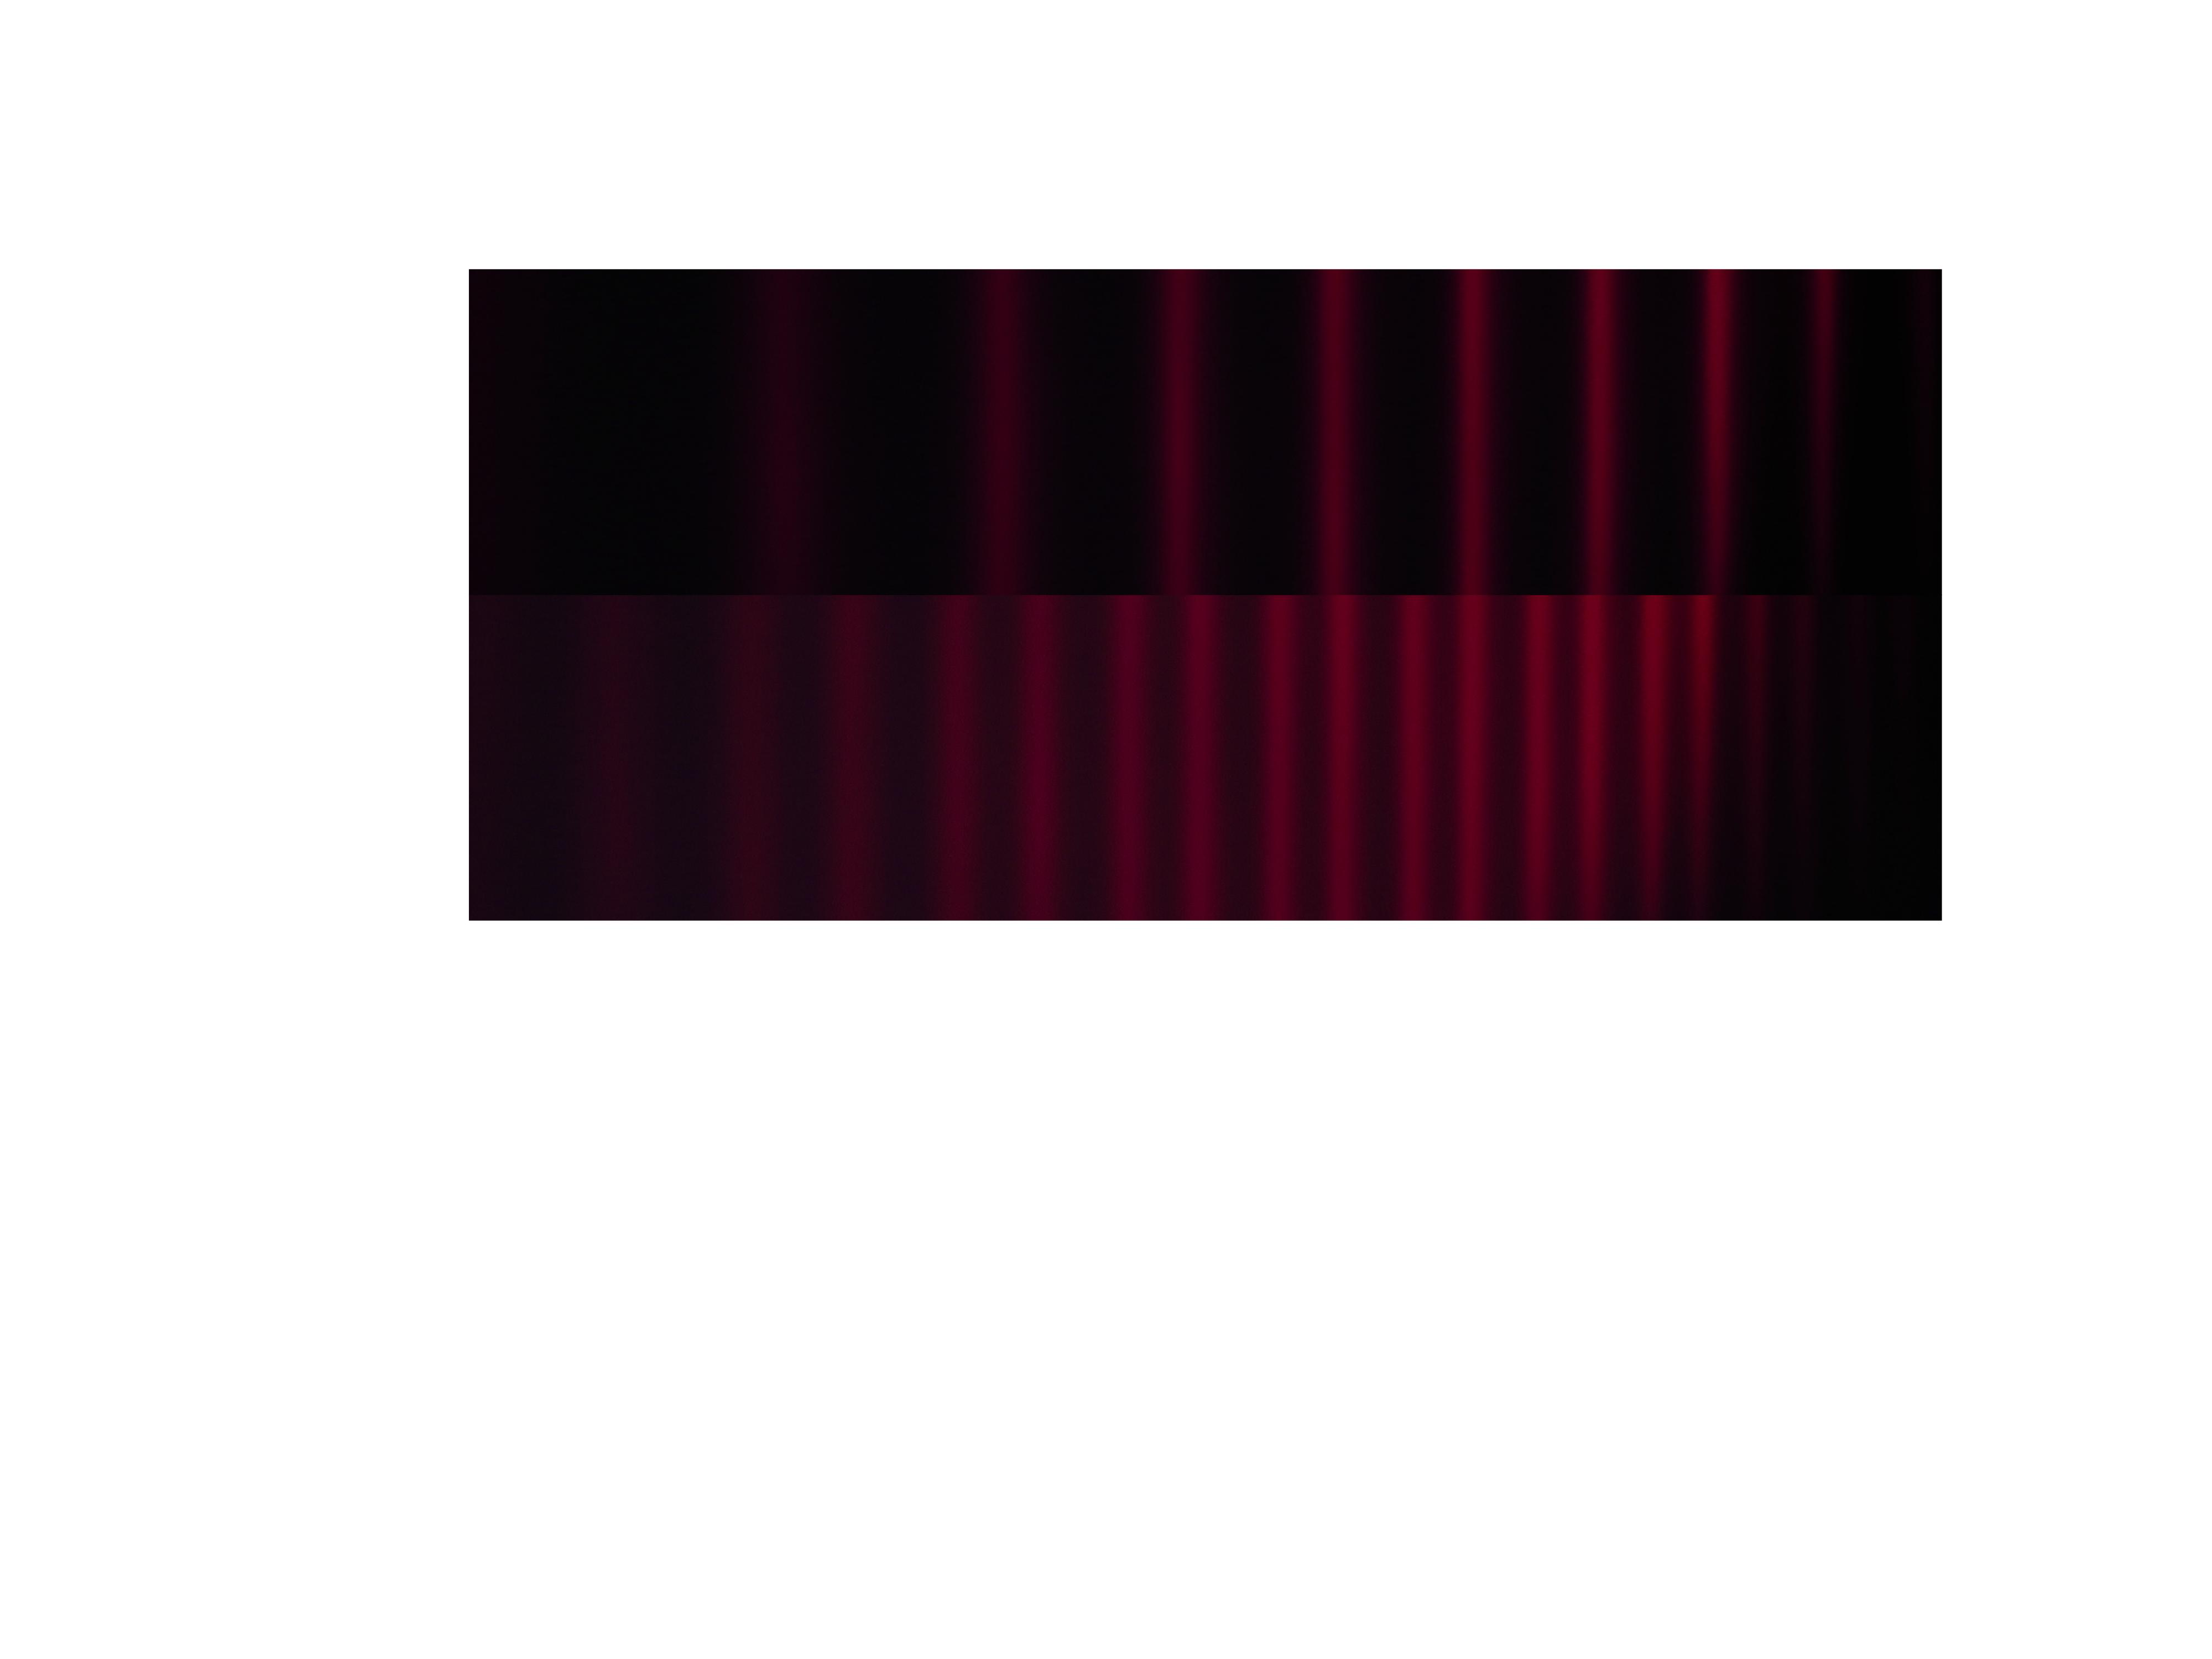
\includegraphics[width=16cm,height=12cm]{Fotos/V27_1.jpg}
	\caption{Magnetischer Flussdichte gegen Stromstärke aufgetragen}
	\label{plot:1}
\end{figure}

\begin{center}
$\delta \lambda$ = (10,29 \pm 0,21) pm
\end{center}

  \subsection{\texorpdfstring{Bestimmung des Lande-Faktors $g_{12}$ der $\pi$-"Uberg"ange f"ur die blaue Linie}{Bestimmung des Lande-Faktors g_12 der pi-"Uberg"ange f"ur die blaue Linie}}
  
        \begin{table}[H] 
	\centering
	\caption{Für die Eichung des Magneten aufgenommene Messwerte des Magnetfeldes neben der zugehörigen Stromstärke} 
	\begin{tabular}{c|c|c|c}

  & $\Delta$ s in px & $\delta s$ in px & $\delta \lambda$ in $10^{-12} m$\\
  \hline 
1&188&92&6,59 \pm 0,24 \\
2&176&84&6,43 \pm 0,25 \\
3&160&72&6,06 \pm 0,28 \\
4&147&63&5,77 \pm 0,30 \\
5&131&58&5,97 \pm 0,34 \\
6&122&52&5,74 \pm 0,36 \\

		
	\end{tabular} 
	  \label{tab:mit}
\end{table} 

\begin{figure}[h]
	\centering
	
\includegraphics[width=16cm,height=12cm]{Fotos/V27_2.jpg}
	\caption{Magnetischer Flussdichte gegen Stromstärke aufgetragen}
	\label{plot:1}
\end{figure}

\begin{center}
$\delta \lambda$ = (6,09 \pm 0,22) pm
\end{center}

  \subsection{\texorpdfstring{Bestimmung des Lande-Faktors $g_{12}$ der $\sigma$-"Uberg"ange f"ur die blaue Linie}{Bestimmung des Lande-Faktors g_{12} der sigma-"Uberg"ange f"ur die blaue Linie}}
  
          \begin{table}[H] 
	\centering
	\caption{Für die Eichung des Magneten aufgenommene Messwerte des Magnetfeldes neben der zugehörigen Stromstärke} 
	\begin{tabular}{c|c|c|c}

  & $\Delta$ s in px & $\delta s$ in px & $\delta \lambda$ in $10^{-12} m$\\
  \hline 
1&178&175&13,25 \pm 0,32 \\
2&172&171&13,40 \pm 0,33\\
3&160&165&13,90 \pm 0,36\\
4&144&153&14,32 \pm 0,41\\
5&124&142&15,43 \pm 0,50\\
6&118&135&15,42 \pm 0,52\\
7&111&127&15,42 \pm 0,55 \\

		
	\end{tabular} 
	  \label{tab:mit}
\end{table} 

\begin{figure}[h]
	\centering
	
\includegraphics[width=16cm,height=12cm]{Fotos/V27_3.jpg}
	\caption{Magnetischer Flussdichte gegen Stromstärke aufgetragen}
	\label{plot:1}
\end{figure}

\begin{center}
$\delta \lambda$ = (14,45 \pm 0,25) pm
\end{center}


  \subsection{\texorpdfstring{Berechnung der experimentellen Lande-Faktoren $g_{ij}$ aus den Abst"anden $\Delta s$ und $\delta s$ der erhaltenen Aufnahmen}{Berechnung der experimentellen Lande-Faktoren g_{ij} aus den Abst"anden Delta s und delta s der erhaltenen Aufnahmen}}

  $\Delta s$ ist der Abstand der benachbarten Interferentzmaxima in der Aufnahme ohne Magnetfeld, $\delta s$ ist die Breite der Aufspaltung eines Interferenzmaximas, in der Aufnahme mit angelegtem Magnetfeld mit St"arke $B$.
  Damit ergibt sich f"ur den Wellenl"angenunterschied $\delta \lambda$ zwischen den beiden Energieniveaus des "Ubergangs
  \begin{equation}
    \delta \lambda = \frac{1}{2}\frac{\delta s}{\Delta s} \Delta \lambda \; .
  \end{equation}
  Mit
  \begin{align}
    \begin{split}
    \frac{\partial E}{\partial \lambda} = \frac{\delta E}{\delta \lambda} &= \frac{\delta}{\delta \lambda} \frac{hc}{\lambda} = -\frac{hc}{\lambda^2}\\
    \iff \delta E &= \frac{ch}{\lambda^2} \delta \lambda
   \end{split}
  \end{align}
  folgt f"ur den Lande-faktor $g_{12}$ mit der Energieniveaudifferenz $\delta E$/Wellenl"angendifferenz $\delta \lambda$ nach Formel (\ref{g_ij}) der Zusammenhang
  \begin{equation}
    g_{12}=\frac{\delta E}{\mu_BB}=\frac{hc\delta \lambda}{\lambda^2\mu_BB} \; .
  \end{equation}

          \begin{table}[H] 
	\centering
	\caption{Für die Eichung des Magneten aufgenommene Messwerte des Magnetfeldes neben der zugehörigen Stromstärke} 
	\begin{tabular}{c|c|c|c|c}

  $\lambda$ pm & B mT & Übergang & $g_{ij,exp}$& $g_{ij,theo}$\\
  \hline 
643,8 &&$\sigma$&&1\\
480 &&$\sigma$&&1,75\\
480 &&$\pi$&&0,01\\


		
	\end{tabular} 
	  \label{tab:mit}
\end{table} 




















\section{Diskussion}

Nach \textcite{demtroeder:exp1} liegt der Wert für der Elastizitätsmodul
von Aluminium bei \SI{71}{\kilo\newton\per\milli\metre^2} und der von
Stahl bei \SI{200}{\kilo\newton\per\milli\metre^2}.  Der in diesem
Protokoll bestimmte Wert für der Elastizitätsmodul von Aluminium beträgt
ca. \SI{73}{\kilo\newton\per\milli\metre^2} und weicht somit um
ca. \SI{2.1}{\percent} vom gefundenen Literaturwert ab.  Bei Stahl
ergibt sich somit bei einem bestimmten Wert von
ca. \SI{1078}{\kilo\newton\per\milli\metre^2} eine Abweichung von
\SI{439}{\percent}. Dieser Wert weicht so stark vom Literaturwert ab,
dass man es nur damit erklären kann, dass während der Vermessung des
Stabes die Messwerte falsch abgelesen wurden.  Der Wert für der
Elastizitätsmodul von Messing liegt nach \textcite{peter-brehm} zwischen
\SI{78}{\kilo\newton\per\milli\metre^2} und
\SI{123}{\kilo\newton\per\milli\metre^2}. Der Mittelwert der beiden
gefundenen Werte für Messing beträgt
ca. \SI{151,6}{\kilo\newton\per\milli\metre^2}. Somit ergibt sich bei
Betrachtung des größten Literaturwertes für der Elastizitätsmodul von
Messing eine Abweichung von ca. \SI{23.3}{\percent} Die relativen Fehler
in Prozent berechnen sich aus den gemessenen Werten $x$ und den
Literaturwerten $x_L$ nach Formel \eqref{eq:rel_fehler}.
%
\begin{equation}
\label{eq:rel_fehler}
\Delta x = 100 \cdot \frac{|x - x_L|}{x_L}    
\end{equation}


% Literaturverzeichnis
\addcontentsline{toc}{section}{Literatur}
\printbibliography
% Anleitung auf jeden Fall zitieren
\nocite{v606}

% \theappendix

\end{document}
